% \begin{figure}[h]
% \centering
% 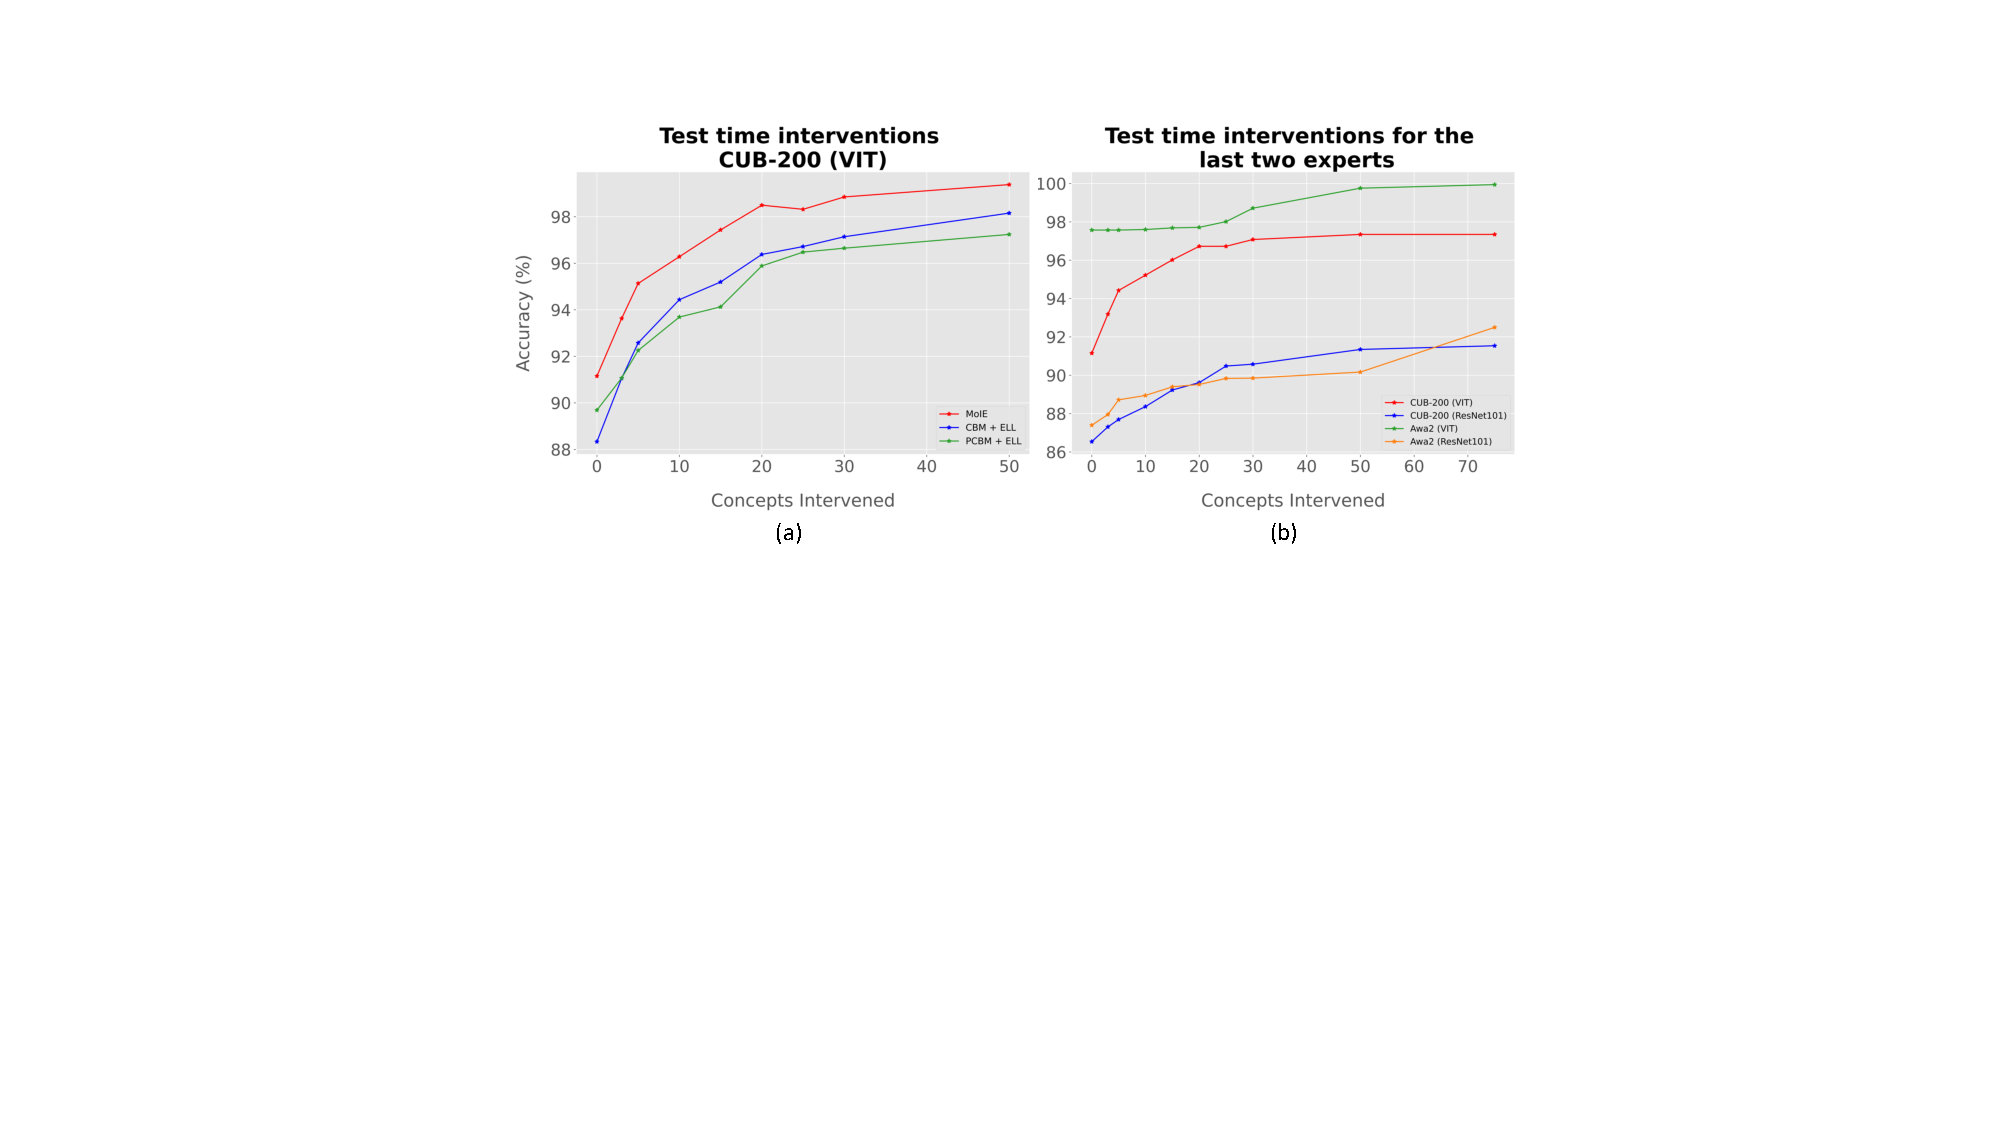
\includegraphics[width=\columnwidth]{figures/main/TTI_expert.pdf}
% \caption{Test time interventions of concepts for (a) on all the samples covered by MoIE, showing MoIE's superior performance over the baselines, (b) on the ``hard'' samples, covered by only the last two experts of MoIE across architectures. All the plots mark the first point on the x-axis as "0," indicating the original model's performance with no intervention.}
% \vskip 0.1in
% \label{fig:tti_expert}
% \end{figure}

\textbf{Comparing with the interpretable-by-design baselines:}~\cref{tab:performance} shows that MoIE achieves comparable performance to the Blackbox. Recall that ``MoIE'' refers to the mixture of all interpretable experts ($g$) only excluding any residuals.
% Also, interpretable-by-design models can not be directly constructed for HAM10000 and ISIC as they have no concept annotation~\cite{yuksekgonul2022post}.
MoIE outperforms the interpretable-by-design baselines for all the datasets except Awa2. Since Awa2 is designed for zero-shot learning, its rich concept annotation makes it appropriate for interpretable-by-design models. In general, VIT-derived MoIEs perform better than their ResNet-based variants.

\textbf{Comparing with the PCBMs:}~\cref{tab:performance} shows that interpretable MoIE outperforms the interpretable posthoc baselines -- PCBM and PCBM + E-LEN for all the datasets, especially by a significant margin for CUB-200 and ISIC.
 We also report ``MoIE + Residual'' as the mixture of interpretable experts plus the final residual to compare with the residualized PCBM, \ie PCBM-h.~\cref{tab:performance} shows that PCBM-h performs slightly better than MoIE + Residual. Note that PCBM-h learns the residual by fitting the complete dataset to fix the interpretable PCBM's mistakes to replicate the performance of the Blackbox, resulting in better performance for PCBM-h than PCBM. However, we assume the Blackbox to be a combination of interpretable and uninterpretable components. So, we train the experts and the final residual to cover the interpretable and uninterpretable portions of the Blackbox respectively. In each iteration, our method learns the residuals to focus on the samples, which are not covered by the respective interpretable experts. Therefore, residuals are not designed to fix the mistakes made by the experts. In doing so, the final residual in MoIE + Residual covers the ``hardest'' examples, lowering its overall performance compared to MoIE. 
% Note that we could not plot auroc for the other datasets that are performing multi-class 
% classification